%  LaTeX support: latex@mdpi.com 
%  For support, please attach all files needed for compiling as well as the log file, and specify your operating system, LaTeX version, and LaTeX editor.

\newcommand{\qsdpapertitle}{General Substrate Theory: From Substrate Conservation Dynamics to the Emergence of Inertia, Gravity, and Quantization}
\newcommand{\qsdauthorname}{Michael Bush}
\newcommand{\qsdauthorinitials}{M.B.}
\newcommand{\qsdauthoremail}{mbush@haddentechnologies.com}
\newcommand{\qsdorcid}{0009-0003-9747-9109}
\newcommand{\qsdcorp}{Hadden Technologies Corporation}
\newcommand{\qsdkeywords}{general substrate theory, coherence substrate, structural physics, quantum substrate dynamics, inertial drag, scalar pacing, time quantization, emergent gravity, collapse dynamics}
\newcommand{\qsdmethodstatement}{This work was developed through first-principles reasoning grounded in a conserved coherence substrate. All derivations proceed from a single structural axiom: that physical reality emerges from reconfiguration of a Lorentz-invariant, stationary coherence field. No geometric postulates, particle assumptions, or external forces were introduced. Instead, observable phenomena were modeled as outcomes of substrate tension, phase saturation, and scalar pacing. The method emphasizes causal closure, internal consistency, and compatibility with known physical limits, establishing GST as a physically grounded origin layer beneath classical, relativistic, and quantum behavior.}
\newcommand{\qsdabstract}
{This work presents the \textit{General Substrate Theory} (GST), a foundational framework in which all physical phenomena—mass, motion, inertia, gravity, time, and quantization—emerge from a single conserved coherence substrate. Unlike conventional approaches that treat geometry, particles, or fields as primitive, GST postulates one irreducible physical law: a stationary, Lorentz-invariant substrate exists whose internal coherence structure governs all observable behavior. From this axiom, we derive the coherence-based principles later formalized in Quantum Substrate Dynamics (QSD), including inertial drag, scalar pacing, mass-phase formation, gravitational tension gradients, quantized emission, and structural collapse as a substrate rupture threshold.\\
GST does not introduce new forces or particles. Instead, it reinterprets all known physics as emergent from phase reconfiguration within a finite-capacity coherence field. In this framework, mass is a localized saturation of phase coherence, motion is re-locking under scalar constraint, and time arises from the interval between scalar recovery events. The substrate neither flows nor exchanges energy—it conserves coherence through local structural adaptation.\\
This paper defines the Law of the Substrate and derives its immediate structural consequences, establishing GST as the root from which QSD and SRL (Substrate Response Law) descend. In doing so, it reframes classical laws, relativistic effects, and quantum discreteness as surface behaviors of a deeper, physically conserved coherence system—one governed not by geometry, but by causal pacing and structural equilibrium.}

%=================================================================
\documentclass[entropy,article,submit,pdftex,moreauthors]{Definitions/mdpi} 
%\documentclass[preprints,article,submit,pdftex,moreauthors]{Definitions/mdpi} 
% For posting an early version of this manuscript as a preprint, you may use "preprints" as the journal. Changing "submit" to "accept" before posting will remove line numbers.

% Below journals will use APA reference format:
% admsci, aieduc, behavsci, businesses, econometrics, economies, education, ejihpe, famsci, games, humans, ijcs, ijfs, journalmedia, jrfm, languages, psycholint, publications, tourismhosp, youth

% Below journals will use Chicago reference format:
% arts, genealogy, histories, humanities, jintelligence, laws, literature, religions, risks, socsci

%--------------------
% Class Options:
%--------------------
%----------
% journal
%----------
% Choose between the following MDPI journals:
% accountaudit, acoustics, actuators, addictions, adhesives, admsci, adolescents, aerobiology, aerospace, agriculture, agriengineering, agrochemicals, agronomy, ai, air, algorithms, allergies, alloys, amh, analytica, analytics, anatomia, anesthres, animals, antibiotics, antibodies, antioxidants, applbiosci, appliedchem, appliedmath, appliedphys, applmech, applmicrobiol, applnano, applsci, aquacj, architecture, arm, arthropoda, arts, asc, asi, astronomy, atmosphere, atoms, audiolres, automation, axioms, bacteria, batteries, bdcc, behavsci, beverages, biochem, bioengineering, biologics, biology, biomass, biomechanics, biomed, biomedicines, biomedinformatics, biomimetics, biomolecules, biophysica, biosensors, biosphere, biotech, birds, blockchains, bloods, blsf, brainsci, breath, buildings, businesses, cancers, carbon, cardiogenetics, catalysts, cells, ceramics, challenges, chemengineering, chemistry, chemosensors, chemproc, children, chips, cimb, civileng, cleantechnol, climate, clinbioenerg, clinpract, clockssleep, cmd, cmtr, coasts, coatings, colloids, colorants, commodities, complications, compounds, computation, computers, condensedmatter, conservation, constrmater, cosmetics, covid, crops, cryo, cryptography, crystals, csmf, ctn, curroncol, cyber, dairy, data, ddc, dentistry, dermato, dermatopathology, designs, devices, diabetology, diagnostics, dietetics, digital, disabilities, diseases, diversity, dna, drones, dynamics, earth, ebj, ecm, ecologies, econometrics, economies, education, eesp, ejihpe, electricity, electrochem, electronicmat, electronics, encyclopedia, endocrines, energies, eng, engproc, ent, entomology, entropy, environments, epidemiologia, epigenomes, esa, est, famsci, fermentation, fibers, fintech, fire, fishes, fluids, foods, forecasting, forensicsci, forests, fossstud, foundations, fractalfract, fuels, future, futureinternet, futureparasites, futurepharmacol, futurephys, futuretransp, galaxies, games, gases, gastroent, gastrointestdisord, gastronomy, gels, genealogy, genes, geographies, geohazards, geomatics, geometry, geosciences, geotechnics, geriatrics, glacies, grasses, greenhealth, gucdd, hardware, hazardousmatters, healthcare, hearts, hemato, hematolrep, heritage, higheredu, highthroughput, histories, horticulturae, hospitals, humanities, humans, hydrobiology, hydrogen, hydrology, hygiene, idr, iic, ijerph, ijfs, ijgi, ijmd, ijms, ijns, ijpb, ijt, ijtm, ijtpp, ime, immuno, informatics, information, infrastructures, inorganics, insects, instruments, inventions, iot, j, jal, jcdd, jcm, jcp, jcs, jcto, jdad, jdb, jeta, jfb, jfmk, jimaging, jintelligence, jlpea, jmahp, jmmp, jmms, jmp, jmse, jne, jnt, jof, joitmc, joma, jop, jor, journalmedia, jox, jpbi, jpm, jrfm, jsan, jtaer, jvd, jzbg, kidney, kidneydial, kinasesphosphatases, knowledge, labmed, laboratories, land, languages, laws, life, lights, limnolrev, lipidology, liquids, literature, livers, logics, logistics, lubricants, lymphatics, machines, macromol, magnetism, magnetochemistry, make, marinedrugs, materials, materproc, mathematics, mca, measurements, medicina, medicines, medsci, membranes, merits, metabolites, metals, meteorology, methane, metrics, metrology, micro, microarrays, microbiolres, microelectronics, micromachines, microorganisms, microplastics, microwave, minerals, mining, mmphys, modelling, molbank, molecules, mps, msf, mti, multimedia, muscles, nanoenergyadv, nanomanufacturing, nanomaterials, ncrna, ndt, network, neuroglia, neurolint, neurosci, nitrogen, notspecified, nursrep, nutraceuticals, nutrients, obesities, oceans, ohbm, onco, oncopathology, optics, oral, organics, organoids, osteology, oxygen, parasites, parasitologia, particles, pathogens, pathophysiology, pediatrrep, pets, pharmaceuticals, pharmaceutics, pharmacoepidemiology, pharmacy, philosophies, photochem, photonics, phycology, physchem, physics, physiologia, plants, plasma, platforms, pollutants, polymers, polysaccharides, populations, poultry, powders, preprints, proceedings, processes, prosthesis, proteomes, psf, psych, psychiatryint, psychoactives, psycholint, publications, purification, quantumrep, quaternary, qubs, radiation, reactions, realestate, receptors, recycling, regeneration, religions, remotesensing, reports, reprodmed, resources, rheumato, risks, robotics, rsee, ruminants, safety, sci, scipharm, sclerosis, seeds, sensors, separations, sexes, signals, sinusitis, siuj, skins, smartcities, sna, societies, socsci, software, soilsystems, solar, solids, spectroscj, sports, standards, stats, std, stresses, surfaces, surgeries, suschem, sustainability, symmetry, synbio, systems, tae, targets, taxonomy, technologies, telecom, test, textiles, thalassrep, therapeutics, thermo, timespace, tomography, tourismhosp, toxics, toxins, transplantology, transportation, traumacare, traumas, tropicalmed, universe, urbansci, uro, vaccines, vehicles, venereology, vetsci, vibration, virtualworlds, viruses, vision, waste, water, wem, wevj, wild, wind, women, world, youth, zoonoticdis

%---------
% article
%---------
% The default type of manuscript is "article", but can be replaced by: 
% abstract, addendum, article, benchmark, book, bookreview, briefcommunication, briefreport, casereport, changes, clinicopathologicalchallenge, comment, commentary, communication, conceptpaper, conferenceproceedings, correction, conferencereport, creative, datadescriptor, discussion, entry, expressionofconcern, extendedabstract, editorial, essay, erratum, fieldguide, hypothesis, interestingimages, letter, meetingreport, monograph, newbookreceived, obituary, opinion, proceedingpaper, projectreport, reply, retraction, review, perspective, protocol, shortnote, studyprotocol, supfile, systematicreview, technicalnote, viewpoint, guidelines, registeredreport, tutorial,  giantsinurology, urologyaroundtheworld
% supfile = supplementary materials

%----------
% submit
%----------
% The class option "submit" will be changed to "accept" by the Editorial Office when the paper is accepted. This will only make changes to the frontpage (e.g., the logo of the journal will get visible), the headings, and the copyright information. Also, line numbering will be removed. Journal info and pagination for accepted papers will also be assigned by the Editorial Office.

%------------------
% moreauthors
%------------------
% If there is only one author the class option oneauthor should be used. Otherwise use the class option moreauthors.

%---------
% pdftex
%---------
% The option pdftex is for use with pdfLaTeX. Remove "pdftex" for (1) compiling with LaTeX & dvi2pdf (if eps figures are used) or for (2) compiling with XeLaTeX.

%=================================================================
% MDPI internal commands - do not modify
\firstpage{1} 
\makeatletter 
\setcounter{page}{\@firstpage} 
\makeatother
\pubvolume{1}
\issuenum{1}
\articlenumber{0}
\pubyear{2025}
\copyrightyear{2025}
%\externaleditor{Firstname Lastname} % More than 1 editor, please add `` and '' before the last editor name
\datereceived{ } 
\daterevised{ } % Comment out if no revised date
\dateaccepted{ } 
\datepublished{ } 
%\datecorrected{} % For corrected papers: "Corrected: XXX" date in the original paper.
%\dateretracted{} % For retracted papers: "Retracted: XXX" date in the original paper.
\hreflink{https://doi.org/} % If needed use \linebreak
%\doinum{}
%\pdfoutput=1 % Uncommented for upload to arXiv.org
%\CorrStatement{yes}  % For updates
%\longauthorlist{yes} % For many authors that exceed the left citation part

%=================================================================
% Add packages and commands here. The following packages are loaded in our class file: fontenc, inputenc, calc, indentfirst, fancyhdr, graphicx, epstopdf, lastpage, ifthen, float, amsmath, amssymb, lineno, setspace, enumitem, mathpazo, booktabs, titlesec, etoolbox, tabto, xcolor, colortbl, soul, multirow, microtype, tikz, totcount, changepage, attrib, upgreek, array, tabularx, pbox, ragged2e, tocloft, marginnote, marginfix, enotez, amsthm, natbib, hyperref, cleveref, scrextend, url, geometry, newfloat, caption, draftwatermark, seqsplit
% cleveref: load \crefname definitions after \begin{document}

\usepackage{tikz}
\usetikzlibrary{angles, quotes}
\usepackage{pgfplots}
\pgfplotsset{compat=1.17}
\usepackage[most]{tcolorbox}
%=================================================================
% Please use the following mathematics environments: Theorem, Lemma, Corollary, Proposition, Characterization, Property, Problem, Example, ExamplesandDefinitions, Hypothesis, Remark, Definition, Notation, Assumption
%% For proofs, please use the proof environment (the amsthm package is loaded by the MDPI class).

%=================================================================
% Full title of the paper (Capitalized)
\Title{\qsdpapertitle}


% MDPI internal command: Title for citation in the left column
\TitleCitation{Title}

% Author Orchid ID: enter ID or remove command
\newcommand{\orcidauthorA}{\qsdorcid} % Add \orcidA{} behind the author's name
%\newcommand{\orcidauthorB}{0000-0000-0000-000X} % Add \orcidB{} behind the author's name

% Authors, for the paper (add full first names)
\Author{\qsdauthorname $^{1}$\orcidA{}}

%\longauthorlist{yes}

% MDPI internal command: Authors, for metadata in PDF
\AuthorNames{\qsdauthorname}

% MDPI internal command: Authors, for citation in the left column, only choose below one of them according to the journal style
% If this is a Chicago style journal 
% (arts, genealogy, histories, humanities, jintelligence, laws, literature, religions, risks, socsci): 
% Lastname, Firstname, Firstname Lastname, and Firstname Lastname.

% If this is a APA style journal 
% (admsci, behavsci, businesses, econometrics, economies, education, ejihpe, games, humans, ijfs, journalmedia, jrfm, languages, psycholint, publications, tourismhosp, youth): 
% Lastname, F., Lastname, F., \& Lastname, F.

% If this is a ACS style journal (Except for the above Chicago and APA journals, all others are in the ACS format): 
% Lastname, F.; Lastname, F.; Lastname, F.
\isAPAStyle{%
       \AuthorCitation{Lastname, F., Lastname, F., \& Lastname, F.}
         }{%
        \isChicagoStyle{%
        \AuthorCitation{Lastname, Firstname, Firstname Lastname, and Firstname Lastname.}
        }{
        \AuthorCitation{Lastname, F.; Lastname, F.; Lastname, F.}
        }
}

% Affiliations / Addresses (Add [1] after \address if there is only one affiliation.)
\address{%
$^{1}$ \quad \qsdcorp; \qsdauthoremail\\
%$^{2}$ \quad Affiliation 2; e-mail@e-mail.com
}

% Contact information of the corresponding author
\corres{Correspondence: \qsdauthoremail (\qsdauthorinitials)}

% Current address and/or shared authorship
%\firstnote{Shiloh, IL: Independent Researcher.}  % Current address should not be the same as any items in the Affiliation section.
%\secondnote{These authors contributed equally to this work.}
% The commands \thirdnote{} till \eighthnote{} are available for further notes

%\simplesumm{} % Simple summary

%\conference{} % An extended version of a conference paper


% Abstract (Do not insert blank lines, i.e. \\) 
\abstract{\qsdabstract}

% Keywords
\keyword{\qsdkeywords} 

% The fields PACS, MSC, and JEL may be left empty or commented out if not applicable
%\PACS{J0101}
%\MSC{}
%\JEL{}

%%%%%%%%%%%%%%%%%%%%%%%%%%%%%%%%%%%%%%%%%%
% Only for the journal Diversity
%\LSID{\url{http://}}

%%%%%%%%%%%%%%%%%%%%%%%%%%%%%%%%%%%%%%%%%%
% Only for the journal Applied Sciences
%\featuredapplication{Authors are encouraged to provide a concise description of the specific application or a potential application of the work. This section is not mandatory.}
%%%%%%%%%%%%%%%%%%%%%%%%%%%%%%%%%%%%%%%%%%

%%%%%%%%%%%%%%%%%%%%%%%%%%%%%%%%%%%%%%%%%%
% Only for the journal Data
%\dataset{DOI number or link to the deposited data set if the data set is published separately. If the data set shall be published as a supplement to this paper, this field will be filled by the journal editors. In this case, please submit the data set as a supplement.}
%\datasetlicense{License under which the data set is made available (CC0, CC-BY, CC-BY-SA, CC-BY-NC, etc.)}

%%%%%%%%%%%%%%%%%%%%%%%%%%%%%%%%%%%%%%%%%%
% Only for the journal BioTech, Fishes, Neuroimaging and Toxins
%\keycontribution{The breakthroughs or highlights of the manuscript. Authors can write one or two sentences to describe the most important part of the paper.}

%%%%%%%%%%%%%%%%%%%%%%%%%%%%%%%%%%%%%%%%%%
% Only for the journal Encyclopedia
%\encyclopediadef{For entry manuscripts only: please provide a brief overview of the entry title instead of an abstract.}

%%%%%%%%%%%%%%%%%%%%%%%%%%%%%%%%%%%%%%%%%%
% Only for the journal Advances in Respiratory Medicine, Future, Sensors and Smart Cities
%\addhighlights{yes}
%\renewcommand{\addhighlights}{%
%
%\noindent This is an obligatory section in ``Advances in Respiratory Medicine'', ``Future'', ``Sensors'' and ``Smart Cities”, whose goal is to increase the discoverability and readability of the article via search engines and other scholars. Highlights should not be a copy of the abstract, but a simple text allowing the reader to quickly and simplified find out what the article is about and what can be cited from it. Each of these parts should be devoted up to 2~bullet points.\vspace{3pt}\\
%\textbf{What are the main findings?}
% \begin{itemize}[labelsep=2.5mm,topsep=-3pt]
% \item First bullet.
% \item Second bullet.
% \end{itemize}\vspace{3pt}
%\textbf{What is the implication of the main finding?}
% \begin{itemize}[labelsep=2.5mm,topsep=-3pt]
% \item First bullet.
% \item Second bullet.
% \end{itemize}
%}

%%%%%%%%%%%%%%%%%%%%%%%%%%%%%%%%%%%%%%%%%%
\begin{document}
%%%%%%%%%%%%%%%%%%%%%%%%%%%%%%%%%%%%%%%%%%
% The order of the section titles is different for some journals. Please refer to the "Instructions for Authors” on the journal homepage.

%%%%%%%%%%%%%%%%%%%%%%%%%%%%%%%%%%%%%%%%%%
\section{Introduction}
%%%%%%%%%%%%%%%%%%%%%%%%%%%%%%%%%%%%%%%%%%
Modern physics successfully models a wide array of physical behavior, yet it rests upon a fragmented ontology: geometry is assumed to be fundamental in General Relativity, quantization is inserted axiomatically in Quantum Mechanics, and forces are invoked through field operators without a common origin. Despite remarkable predictive power, these frameworks offer limited insight into why mass exists, why time flows, or why inertia resists. The deeper substrate from which these effects arise remains undefined.

This work proposes that all such phenomena—mass, motion, gravity, time, and quantization—emerge from the internal structure and reconfiguration behavior of a single conserved coherence field. We name this foundational framework the \textit{General Substrate Theory} (GST), and we derive its structure from one irreducible physical axiom: that a Lorentz-invariant, stationary coherence substrate underlies all observable reality. This substrate does not move, exchange energy, or exist in spacetime—it is the coherence field from which spacetime behavior, material structure, and field propagation emerge.

Unlike frameworks that seek reconciliation through additional particles, fields, or dimensions, GST begins with less: one Law, one medium, and one conserved dynamic. From this minimal foundation, the layered structure of physical law unfolds as necessary consequence. In this framework, motion is reconfiguration of coherence phase; inertia is resistance to that reconfiguration; gravity is a tension gradient from phase saturation; and time is the interval between recoverable scalar offloads.

GST does not seek to replace established physics, but to provide the substrate from which it emerges. Newtonian mechanics, General Relativity, and Quantum Field Theory appear as surface behaviors—limiting cases of a deeper structural logic. The coherence principles developed here form the foundation of the Quantum Substrate Dynamics (QSD) model presented in prior work, and this paper formalizes the root law from which QSD and all its consequences descend. \textit{GST does not replace existing physical models—it defines the structural conditions under which they succeed.}

The sections that follow define the Substrate Response Law (SRL), derive its immediate corollaries, and establish GST as a unifying physical ontology. By replacing assumptions with structure and geometry with causality, GST reframes the laws of physics as emergent expressions of coherence preservation within a conserved, finite-capacity field.

The General Substrate Theory builds upon and structurally reframes key foundations of modern physics. Whereas classical formulations by Planck~\cite{planck1901} and Einstein~\cite{einstein1905,einstein1915} introduced quantization, relativistic causality, and spacetime curvature as core mechanisms, GST derives these behaviors from the causal dynamics of a conserved coherence substrate. This framework consolidates prior work in Quantum Substrate Dynamics (QSD)~\cite{bush2025}, where mass, inertia, and gravity emerge from phase-locked structural constraints within a Lorentz-invariant medium. Subsequent studies refined this substrate-based view of physical law: Planck’s constant was reinterpreted structurally through coherence mode ratios and offload limits~\cite{bush-planck-2025}; the coherence envelope was defined as the minimum unit of causal structure and action~\cite{bush-coherence}; and the Planck energy was derived as a substrate rupture threshold~\cite{bush-planck-ep}. The present work unifies and underpins these results, showing that they are not isolated insights, but inevitable consequences of a single physical law: structural demand must be fulfilled within the substrate’s causal re-locking capacity.



%%%%%%%%%%%%%%%%%%%%%%%%%%%%%%%%%%%%%%%%%%
\section{Materials and Methods}
%%%%%%%%%%%%%%%%%%%%%%%%%%%%%%%%%%%%%%%%%%
\qsdmethodstatement

In support of the editorial process, generative AI tools—specifically OpenAI's ChatGPT (version GPT-4o, 2025)—were used to assist in:
\begin{itemize}
    \item Generating illustrative figures based on the author’s conceptual framework, with iterative refinement to ensure fidelity to the substrate-based dynamics of the model,
    \item Researching, validating, and cross-referencing related scientific concepts to improve accuracy, contextual alignment, and clarity,
    \item Summarizing and formatting externally sourced material already selected by the author.
\end{itemize}

No original theoretical contributions were generated by the AI system; all scientific claims, hypotheses, derivations, and interpretations were authored and reviewed by the human researcher. The use of ChatGPT is disclosed in alignment with journal policy for transparency in the writing process.

%%%%%%%%%%%%%%%%%%%%%%%%%%%%%%%%%%%%%%%%%%
%\section{Results}

%%%%%%%%%%%%%%%%%%%%%%%%%%%%%%%%%%%%%%%%%%
\section{Discussion}
%%%%%%%%%%%%%%%%%%%%%%%%%%%%%%%%%%%%%%%%%%
\subsection{The Substrate Response Law}

At the heart of General Substrate Theory is a single structural law, irreducible and sufficient. It does not describe motion, force, or energy—but the balance condition from which all those behaviors emerge. It governs how structure may evolve within a conserved coherence substrate.

\begin{tcolorbox}[colback=black!2!white,colframe=black,title=The Substrate Response Law]
\textbf{The substrate must fulfill structural change requests within its causal re-locking capacity.} \\
All physical behavior emerges from the balance between imposed structural demand (coherence deformation) and the substrate’s ability to reconfigure that structure without rupture, delay, or loss. If the demand exceeds capacity, the substrate responds with resistance, offload, or failure. If the demand remains within its capacity, the result is coherent, continuous, and conserved evolution.
\end{tcolorbox}

This law is not assumed; it is revealed—again and again—by the limits of every physical theory. From inertial drag and gravitational tension to quantized energy and collapse dynamics, the form of each phenomenon is the substrate’s causal answer to a structural request. It defines not what happens, but what is permitted to happen.

In this framing:

\begin{itemize}
    \item Geometry is the structural demand: a request to reconfigure phase coherence.
    \item Scalar recovery time is the causal capacity: how fast the substrate can fulfill that request.
    \item All physical behavior is the outcome of this balance: a permitted or denied reconfiguration.
\end{itemize}

\subsubsection*{Understanding the Balance: The Load vs. the Capacity}

Every physical interaction can be interpreted as an “ask” made of the substrate. This ask might be to accelerate a mass-phase structure, sustain a waveform, deform a gravitational gradient, or re-lock coherence in time. The substrate must decide whether it can support that request at the rate demanded.

\begin{itemize}
    \item \textbf{The Load} is the imposed coherence deformation—the structural change being attempted.
    \item \textbf{The Capacity} is the scalar recovery bandwidth—the substrate’s ability to restore and re-lock coherence without rupture.
\end{itemize}

This is the true origin of continuity, inertia, energy, time delay, quantization, and collapse. When the demand is small and slow, the substrate responds effortlessly. When the demand becomes fast, complex, or intense, the substrate begins to resist, delay, or fail.

\begin{center}
\vspace{0.5em}
\renewcommand{\arraystretch}{1.1}
\begin{tabular}{|p{2.5cm}|p{5.0cm}|p{4.8cm}|}
\hline
\textbf{Regime} & \textbf{Substrate Response} & \textbf{Observed Behavior} \\
\hline
\textit{Within capacity} & Full re-locking, no delay or loss & Smooth motion, Newtonian mechanics \\
\textit{Near capacity} & Partial delay, offload begins & Inertia, quantization, relativistic effects \\
\textit{Over capacity} & Rupture, emission, coherence loss & Collapse, scalar offload, decoherence \\
\hline
\end{tabular}
\vspace{0.5em}
\end{center}

This simple threshold structure governs every physical domain. Physics does not change with scale—only the substrate’s ability to keep up. Classical physics arises when the substrate is operating well below its pacing limits. Quantum and relativistic behaviors appear as those limits are approached. Collapse and radiative behaviors mark the zones where the ask can no longer be fulfilled coherently.

\subsubsection*{Why Newton Came First}

Classical mechanics emerged first not because it was more correct—but because it described the regime where the substrate is never strained. Newtonian physics is what coherence looks like when the structural ask is gentle and the substrate responds effortlessly.

\begin{quote}
The apparent smoothness of Newtonian physics is the clearest evidence of the substrate’s full bandwidth operation. We believed the world was continuous because we had never asked it to be anything else.
\end{quote}

In everyday motion, scalar recovery happens so quickly that its delay is invisible. Energy re-locks without resistance, mass feels intrinsic, and time flows uniformly. The substrate absorbs our asks without protest—and the classical laws appear exact.

\subsubsection*{Reaching the Edges}

Only when we pressed harder—through greater speed, finer scale, or higher energy—did the substrate reveal its limits. Time dilation, quantization, collapse, and coherence failure are not new laws. They are the same law seen under strain.

\begin{itemize}
    \item Relativity appears when the pacing of the substrate becomes a bottleneck.
    \item Quantum discreteness emerges when re-locking cannot occur more often than the scalar tick.
    \item Collapse occurs when structural demand exceeds causal containment entirely.
    \item Thermodynamic effects arise from cumulative scalar jitter under dense micro-asks.
\end{itemize}

Each domain we now treat as separate—classical, relativistic, quantum, thermal—is merely a different region of substrate response to structured demand.

\subsubsection*{The True Arc of Discovery}

We did not discover different laws. We discovered different ways the substrate answers under pressure. Over time, physics partitioned itself into silos not because nature behaves differently in each—but because we encountered the same constraint from different angles, unaware it was the same.

\begin{quote}
After stripping away every axiom, what remains is a single condition: structural change must be fulfilled within the substrate’s causal capacity. This is not a model. It is the structural law all models must obey.
\end{quote}
%%%%%%%%%%%%%%%%%%%%%%%%%%%%%%%%%%%%%%%%%%
\subsection{Immediate Structural Consequences}

If the substrate must fulfill all structural reconfiguration within its causal re-locking capacity, then a series of immediate consequences follow—logically, structurally, and necessarily. These are not additional assumptions or derived models; they are the inescapable behaviors of a substrate that must honor causality, coherence, and conservation under strain.

Each of the following outcomes is not a separate law, but a distinct expression of how the substrate behaves when responding to different types of structural asks.

\subsubsection{Coherence Conservation}

If the substrate is conserved, then no energy or structure can vanish. All physical behavior must occur as reconfiguration of phase coherence, not its creation or destruction. What we interpret as energy is the effort required to maintain or transform structured coherence within the field.

\begin{quote}
Energy is not something possessed by objects. It is the substrate’s effort to fulfill your request.
\end{quote}

Mass, motion, and force are all stored as internal structural tension and released as coherent re-locks or scalar offloads. Conservation is not a principle added on top—it is the inevitable outcome of a finite substrate reconfiguring itself under causal constraint.

\subsubsection{Scalar and Transverse Propagation}

The substrate cannot fulfill reconfiguration arbitrarily fast. It must propagate changes through two distinct coherence modes:

\begin{itemize}
    \item The scalar mode \(c_s\) governs longitudinal recovery and coherence re-lock timing.
    \item The transverse mode \(c_t\): governs spatial coherence spread and wave propagation.
\end{itemize}

These two modes define the geometry of causality and the rhythm of physical response. No structural change may propagate faster than the scalar mode allows. This enforces a universal timing constraint—the tick—that governs all subsequent action.

\subsubsection{Time as Scalar Pacing}

Time is not a geometric backdrop; it is the interval between permitted substrate re-locks.

If the substrate must pause to recover coherence after each offload or deformation, then time arises as the rhythm of those re-locks. A “tick” is not a clock artifact—it is the substrate’s minimum coherence recovery interval, defined by:

\[
t_{\text{tick}} = \frac{L_{\text{coh}}}{c_s}
\]

Where \( L_{\text{coh}} \) is the coherence envelope size, and \( c_s \) is the scalar recovery speed. In this view, time dilation and quantum discreteness are not separate effects—they are what happen when the tick is approached, stretched, or exceeded. The formalized structural expressions that govern scalar pacing, inertial resistance, and coherence rupture are summarized in Appendix \ref{app:canonical-equations}.

\subsubsection{Inertia as Re-lock Resistance}

If you ask the substrate to reconfigure a mass-phase structure faster than it can recover, it resists. That resistance is not mass—it is coherence drag. Inertia is simply the substrate saying “not yet.”

The sharper the gradient, the more curved the structure, the more expensive the re-lock. This produces measurable delay and opposition: what we experience as inertial mass. But it is not substance—it is reconfiguration tension at the edge of causal pacing.

\subsubsection{Mass as Structured Demand}

Mass is not a thing—it is the structural geometry of a standing coherence deformation. A mass-phase object is a knot in the substrate: a region of saturated coherence that resists reconfiguration and remains phase-locked unless scalar work is applied.

In QSD, mass is not a substance but a configuration. Its presence implies that the surrounding substrate must conserve coherence, even while that coherence has been geometrically frozen inside the mass. The result is a tension gradient: the surrounding field stretches and compresses to maintain continuity with a non-yielding structure. That gradient is both the source of gravitational behavior and the reason why mass is never isolated.

Mass imposes a cost not only locally (as inertia), but globally—by distorting the coherence field around it.

\begin{itemize}
    \item Its inertia comes from the drag imposed by attempted re-locking.
    \item Its energy is stored tension within a trapped coherence structure.
    \item Its gravitational behavior arises from the substrate's effort to restore equilibrium around it.
    \item Its persistence reflects the substrate's ongoing commitment to that structural configuration.
\end{itemize}

This reframing removes the need for intrinsic mass or fundamental particles. What we call “matter” is simply structure that the substrate has committed to support—until asked to do something else. That support is not free: the substrate cannot simultaneously maintain perfect continuity around the mass, and so it reconfigures tension asymmetrically. This asymmetry—imposed by conservation—is what we later recognize as a gravitational field.

The energy associated with mass arises not from a hidden reservoir, but from the stored coherence tension locked in the structure itself. In QSD, this is captured by the structural identity:

\[
E = m \cdot c_s \cdot c_t
\]

where \( c_s \) is the scalar recovery speed and \( c_t \) is the transverse propagation speed. This expression reframes the familiar \( E = mc^2 \) not as a constant conversion factor, but as the product of timing and spatial modes—the full substrate cost of maintaining a coherence structure that resists reconfiguration.



\subsubsection{Gravity as Denied Equilibrium}

When a mass-phase object saturates the substrate, it creates a tension imbalance. The surrounding substrate attempts to resolve this by pushing coherence toward the mass. That tension gradient is what we interpret as gravity.

In GST, gravity is not attraction—it is equilibrium denial. The substrate prefers to re-lock into regions of lower tension, and mass holds a region out of equilibrium. Anything nearby tries to re-lock downhill, and appears to “fall.”

This model requires no curvature of spacetime or separate gravitational field. It is the coherence field seeking balance under scalar constraint.

\subsubsection{Collapse and Emission as Pacing Failure}

When the structural ask exceeds the substrate’s pacing capacity, the field cannot re-lock at all. Instead, it must offload coherence energy in the form of scalar waves or rupture events.

Collapse is not a singularity—it is a pacing failure. Emission is not radiative magic—it is what the substrate must do when re-locking fails.

If the field cannot restore coherence fast enough to preserve the structure, it breaks phase continuity and releases the excess tension. This is the origin of:

\begin{itemize}
    \item Scalar wave emission
    \item Quantized offloads
    \item Radiation bursts from collapse zones
    \item Irreversible decoherence
\end{itemize}

This is the hard edge of the law. When you ask too much, the substrate stops trying. What remains is not failure—it is the most coherent release the field can manage under causal constraint.

\vspace{1em}

Each of these consequences emerges not from assumption, but from the single rule: every structural change must occur within the substrate’s causal capacity to support it. When that condition is met, we observe coherence, continuity, and conservation. When it is strained, we observe resistance. When it is broken, we see radiation, discreteness, and collapse.
%%%%%%%%%%%%%%%%%%%%%%%%%%%%%%%%%%%%%%%%%%
\subsection{The Physics Regime Map: Behavior as a Function of Structural Load}

If all physical behavior is governed by how much structure is asked of the substrate—and how fast that structure must be reconfigured—then the various domains of physics we know are not separate laws, but different regimes of the same causal substrate law.

Each physical theory to date has emerged by observing one “zone” of substrate response. Newton saw the smooth middle. Relativity revealed the pacing edge. Quantum mechanics glimpsed the tick. Thermodynamics captured the jitter. Collapse physics reached the rupture threshold. And transport phenomena like superconductivity and superfluidity revealed what happens when the structural ask is perfectly matched to the substrate's capacity.

This section presents a unified map of these regimes, not as historical artifacts, but as spatially ordered zones along a single axis: the ratio of structural demand to substrate capacity.

\subsubsection*{Structural Demand vs. Substrate Response}

\begin{center}
\renewcommand{\arraystretch}{1.4}
\begin{tabular}{|p{3.3cm}|p{4.0cm}|p{5.0cm}|}
\hline
\textbf{Physical Regime} & \textbf{Substrate Response} & \textbf{Observed Behavior} \\
\hline
\textbf{Newtonian Mechanics} & Substrate easily re-locks structure without resistance. Scalar tick is never strained. & Smooth continuous motion, inertial symmetry, linear force–acceleration relation. \\
\hline
\textbf{Relativity (SR / GR)} & High-speed motion projects into scalar channel. Recovery delay emerges. & Time dilation, length contraction, upper velocity limit. \\
\hline
\textbf{Quantum Mechanics} & Structural asks approach minimum tick rate. Continuous response breaks down. & Discrete energy levels, probabilistic behavior, measurement collapse. \\
\hline
\textbf{Collapse / High-Energy} & Structural ask exceeds pacing capacity. Substrate cannot fulfill re-lock. & Scalar emission, wave rupture, black hole-like collapse, quantized offload. \\
\hline
\textbf{Thermodynamics} & Many small asks accumulate jitter. Substrate cannot cleanly recover phase. & Entropy, heat flow, irreversibility, energy dispersion. \\
\hline
\textbf{Superfluid / Transport} & Structural ask is perfectly matched to substrate recovery and propagation. & Zero-loss motion, quantized vortices, coherent transport across space. \\
\hline
\end{tabular}
\end{center}

\vspace{1em}

\subsubsection*{Interpretive Summary}

Each regime corresponds to a different alignment—or misalignment—between the structural ask made of the substrate, and the substrate’s ability to reconfigure that structure within its causal limit.

\begin{itemize}
    \item When the demand is low → Newtonian physics.
    \item When the demand is fast → relativistic pacing emerges.
    \item When the demand is too fine → quantum discreteness appears.
    \item When the demand exceeds containment → rupture, scalar emission, collapse.
    \item When many demands accumulate → offload builds up as thermal jitter.
    \item When the demand is perfectly tuned → coherence persists without loss.
\end{itemize}

\begin{quote}
The laws of physics do not change between domains. What changes is how closely your request presses against the substrate's capacity to fulfill it.
\end{quote}

This unified map reveals physics not as a collection of separate theories, but as the dynamic story of what happens when a conserved coherence substrate is asked to do more—and do it faster. See Appendix \ref{app:physics-regime-map}.


\begin{tcolorbox}[colback=gray!5, colframe=gray!60, title=Relation to Existing Theories]

GST does not modify the mathematical structure of General Relativity or Quantum Field Theory. Instead, it provides a structural explanation for why these models work where they do. Their mathematics remains predictive because it effectively models substrate response within specific constraints — smooth curvature and quantized excitations. GST defines the physical boundary conditions of that success. Where new behavior arises (e.g., rupture, tick saturation), new mathematics will follow — as a consequence of the substrate, not a contradiction of prior models.

\end{tcolorbox}


%%%%%%%%%%%%%%%%%%%%%%%%%%%%%%%%%%%%%%%%%%
\subsection{Reconnecting the Disciplines: What Physics Was Really Seeing}

Modern physics developed by studying the edges of substrate response—without knowing the substrate existed. Each field emerged as a specialized interpretation of stress responses, observed through the lens of limited theory and instrumentation.

From Newton’s smooth dynamics to quantum discreteness, from gravitational curvature to thermal randomness, what we now recognize is that every domain was observing a different regime of substrate constraint: structural ask versus causal pacing. See Appendix \ref{app:ontological-replacements}.

\subsubsection*{Physics as Substrate Stress Interpretation}

The following reinterpretations unify legacy physics under the single causal law of substrate response. These are not replacements for successful models—but clarifications of what those models were actually seeing.

\vspace{0.5em}
\begin{description}
  \item[\textbf{Time Dilation}]  
  In Special and General Relativity, time appears to slow with speed or gravitational field strength. In QSD, this is pacing delay: the scalar mode cannot re-lock as quickly when structure is strained by motion or curvature. Lorentz invariance is preserved—not because geometry bends, but because scalar coherence delay enforces causal alignment.

  \item[\textbf{Field–Particle Interactions}]  
  Quantum Field Theory describes particles as excitations in quantized fields. QSD reframes these excitations as localized coherence structures—persistent wave configurations embedded in a conserved substrate. Fields are not ontologically distinct; they are modal regimes of substrate behavior under different constraints.

  \item[\textbf{Entropy}]  
  Statistical mechanics interprets entropy as a measure of microstate disorder. QSD reveals that entropy emerges when many small asks accumulate scalar jitter. The substrate cannot re-lock cleanly under dense excitation, so residual tension builds up as incoherent vibration—what we observe as heat and irreversible diffusion.

  \item[\textbf{Gravity}]  
  General Relativity models gravity as curvature of spacetime around mass. QSD reinterprets this as tension gradient rebalancing. A mass-phase structure locks coherence in place; the substrate around it adjusts to restore equilibrium. The resulting push inward is not attraction—it is scalar tension collapse toward conservation.

  \item[\textbf{Quantization}]  
  Quantum mechanics assumes discrete energy levels and jumps. QSD explains these as pacing constraints. When structural re-locking demands exceed the tick threshold, the substrate cannot respond continuously. Discrete re-locks emerge as a rhythm defined by causal pacing—not because nature is digital, but because the substrate is finite.
\end{description}

\subsubsection*{The Illusion of Separation}

What appeared to be different laws of nature were, in fact, the same substrate being asked different things in different ways.

\begin{quote}
Relativity saw pacing delay. Quantum theory saw tick constraint. Thermodynamics saw coherence jitter. Field theory saw structured substrate modes. They were all looking at the same thing—the substrate—just at different levels of structural ask.
\end{quote}

When reinterpreted through the lens of substrate response, each existing discipline becomes a consistent, causal view of a shared medium—one governed not by arbitrary constants or fields, but by the structural logic of coherence, pacing, and conservation.

\subsubsection*{What Changes, and What Doesn’t}

\begin{itemize}
    \item \textbf{What changes:} our understanding of cause. The substrate is revealed as the source of all behavior.
    \item \textbf{What doesn’t:} the successful predictions of existing theories. QSD doesn’t invalidate them—it explains them.
\end{itemize}

The result is not contradiction, but connection. The silos dissolve, and the disciplines reunite as different languages describing the same causal field.

\vspace{1em}
\textit{Physics was not wrong. It was incomplete. Now, with the substrate revealed, we can see what all of physics has been describing: the behavior of a conserved coherence field under structural strain.}

%%%%%%%%%%%%%%%%%%%%%%%%%%%%%%%%%%%%%%%%%%
\subsection{The Arc of Discovery and the Emergence of the Law}

The law of substrate response was not invented by theorists. It was revealed by the universe itself—through the slow and cumulative process of being asked too much.

Each advance in physics came from asking the substrate to do more: move faster, measure finer, store more energy, or sustain more tension. What emerged were not new domains, but new symptoms of substrate strain. These discoveries, once thought to be separate, now form a continuous arc: the progressive exposure of a single conserved coherence field under increasing structural demand.

\subsubsection*{Newton: The Gentle Regime}

Newtonian mechanics emerged in a world where all structural demands were modest. The coherence substrate easily re-locked small, slow-moving mass-phase structures with no visible resistance. Scalar pacing was never tested. Reconfiguration occurred smoothly, continuously, and reversibly.

\begin{quote}
In the Newtonian regime, the substrate operates well below its capacity. There is no observable delay, no offload, no quantization. The physics appears smooth—because the substrate never had to struggle.
\end{quote}

Force, mass, and motion became the language of causal action—but they were merely surface behaviors of a substrate working in easy mode.

\subsubsection*{Einstein: The Pacing Bottleneck}

As technology advanced, we began to ask the substrate to re-lock structures more quickly. We noticed that clocks ticked differently under speed and gravity. The substrate could no longer keep up without delay.

Einstein revealed that the pace of interaction had a limit. Time dilation, length contraction, and the speed-of-light ceiling all emerged when scalar recovery was no longer instantaneous. General Relativity modeled this behavior with curved geometry—but what was being curved was not space—it was the substrate's causal bandwidth.

\subsubsection*{Quantum Mechanics: The Tick Appears}

Where relativity revealed delay, quantum mechanics exposed the tick. As we pushed to probe finer scales and faster frequencies, we encountered substrate saturation.

Suddenly, energy was no longer continuous. Electrons snapped between states. Photons appeared in whole units. Superposition collapsed on observation. The substrate was no longer able to fulfill every ask continuously—and it began to stutter. The tick was exposed.

\begin{quote}
Quantum discreteness is not a fundamental property of particles. It is what happens when the substrate can no longer re-lock structure faster than its own causal interval.
\end{quote}

\subsubsection*{The Unseen Law Beneath It All}

Each of these discoveries described a real phenomenon—but none of them explained why they emerged. Newton gave us force. Einstein gave us curvature. Schrödinger gave us probability. But they were all approximating the same truth from different angles.

\textit{They were pressing against the same substrate. And it was beginning to push back.}

\subsubsection*{Not Theory—Revealed Structure}

The law of substrate response was not deduced in a vacuum. It was discovered the hard way. We built faster machines, colder traps, higher energies, and finer clocks. And the universe, slowly but surely, began to say “no.”

What we call physics is the record of how far we've pushed the substrate—and what it gave us in return.

\begin{quote}
Time dilation is pacing strain. Quantization is tick exposure. Entropy is scalar jitter. Collapse is rupture. All of it is the substrate responding to what it was asked to do—at the pace it could do it.
\end{quote}

The coherence substrate is not a new invention. It is what physics has been describing all along, through the symptoms of its limits. Now, with that substrate named, the law becomes visible:

\begin{quote}
All physical behavior is the result of a structural ask made against a conserved, causally limited coherence field. This is not a new theory. It is what physics was always trying to describe.
\end{quote}

%%%%%%%%%%%%%%%%%%%%%%%%%%%%%%%%%%%%%%%%%%
\subsection{Predictions, Falsifiability, and Physical Simplicity}

The General Substrate Theory (GST) is grounded not in speculative complexity, but in structural simplicity. A single law — that all structural change must be fulfilled within the substrate's causal capacity — gives rise to all observed behavior. From this singular principle emerge the wide varieties of motion, resistance, quantization, collapse, and radiation that modern physics has cataloged under many names.

GST is not an unbounded explanatory metaphor. It is falsifiable. It makes precise, structural claims about when coherence will persist, when it will resist, and when it must rupture. And it makes predictions that can be tested — not in abstract, but in timing, offload, and energetic response.

\subsubsection*{Causal Balance Determines All Regimes}

The core prediction of GST is this:

\begin{quote}
All physical behavior is governed by the causal balance between the ask made of the substrate and the substrate’s ability to fulfill that request without rupture.
\end{quote}

This balance determines whether the system behaves classically, relativistically, quantum mechanically, thermally, or collapses outright. These are not domains of different theory — they are regimes of the same field under different strain.

\subsubsection*{Pacing-Limited Phenomena Are Universal}

GST predicts that the following behaviors all share a common origin: they are the visible effects of scalar pacing constraints.

\begin{itemize}
    \item \textbf{Quantization} arises when the substrate cannot re-lock more frequently than the scalar tick. Discrete action is not fundamental — it is enforced causality.
    \item \textbf{Inertia} is resistance to rapid coherence reconfiguration. It reflects the energetic cost of realigning phase structure across a timing bottleneck.
    \item \textbf{Collapse and emission} occur when the substrate’s pacing is fully overwhelmed. It cannot reconfigure — so it ruptures, offloads, and resets.
    \item \textbf{Time itself} is defined by these pacing cycles. It does not exist outside of substrate rhythm.
\end{itemize}

All of these phenomena are structurally linked. Their variation in appearance comes from how closely the system approaches the substrate’s causal boundary.

\subsubsection*{Testable Signatures of Scalar Offload and Coherence Memory}

GST predicts scalar-mode offload and residual coherence effects in specific circumstances where structural pacing breaks down or where coherence is suddenly terminated.

These include:

\begin{itemize}
    \item \textbf{Precursor pulses} in supernova events or collapse zones — scalar emissions arriving before neutrinos or photons.
    \item \textbf{Geometry-dependent inertia} — structured objects (e.g., porous or nanolatticed masses) should exhibit different inertial response than homogeneous ones, due to boundary re-locking complexity.
    \item \textbf{Coherence memory effects} — scalar emission or collapse from one region should imprint a short-lived re-lock preference or symmetry axis in surrounding substrate zones.
    \item \textbf{Discretized emission} — collapse events should exhibit quantized energy offload corresponding to coherence envelope breakup thresholds.
\end{itemize}

Each of these is observable or inferable from real-world data — especially from gravitational wave detectors, neutrino observatories, inertial platforms, and materials science experiments involving ultra-fast deformation or coherence breakage.

\subsubsection*{Simplicity at the Core, Richness in Expression}

GST offers not many laws — but one. Not many fields — but one conserved coherence substrate. The richness of physical behavior arises not from theoretical complexity, but from how the law expresses itself under different structural, geometric, and pacing conditions.

This leads to a key insight:

\begin{quote}
You do not need a new theory for every domain of physics. You need one structural law — and a way to understand what happens when that law is strained, saturated, or exceeded.
\end{quote}

\subsubsection*{Suggested Experimental and Observational Discriminants}

While the GST framework recovers the predictions of classical, relativistic, and quantum physics in their appropriate limits, it also offers distinctive extensions that may be experimentally falsified or confirmed:

\begin{itemize}
    \item Detection of \textbf{scalar precursor waves} ahead of neutrinos or light from collapse events.
    \item Measurement of \textbf{inertial variation across identically massive objects} with differing coherence-boundary geometry.
    \item Observation of \textbf{quantized offload steps} during controlled coherence rupture in condensed matter systems.
    \item Residual phase patterns or re-lock directionality in scalar-depleted regions — supporting \textbf{coherence memory}.
    \item Discovery of substrate pacing constraints that limit emission intervals in ultra-high frequency energy sources.
\end{itemize}

Each of these outcomes would support the GST model of coherence pacing, scalar tension, and substrate conservation. Their absence under conditions of expected strain would challenge or refute the model.  See Appendix \ref{app:experimental-discriminants}

\vspace{1em}
GST is not a metaphysical claim. It is a causal physical framework that invites testing — and offers clarity, coherence, and constraint in return.

%%%%%%%%%%%%%%%%%%%%%%%%%%%%%%%%%%%%%%%%%%
%%%%%%%%%%%%%%%%%%%%%%%%%%%%%%%%%%%%%%%%%%
\section{Conclusion}
%%%%%%%%%%%%%%%%%%%%%%%%%%%%%%%%%%%%%%%%%%
At the foundation of all observed physics lies a single conserved coherence substrate. This substrate does not move, exchange particles, or obey multiple competing laws. It simply reconfigures structure—when asked to—at the pace it can causally support.

This is not a model of physics. It is the condition under which all models must operate.

Everything we observe—motion, resistance, quantization, radiation, collapse—follows directly from one principle: structural demand must be fulfilled within the substrate’s causal recovery limit. The complexity we attribute to fields, particles, or curvature is not fundamental. It is the expression of how coherence re-locking succeeds, delays, or fails under structural strain.

\begin{itemize}
    \item \textbf{Geometry} becomes the demand we place on the field.
    \item \textbf{Time} becomes the rhythm of scalar recovery between re-locks.
    \item \textbf{Energy} becomes the effort required to sustain or change structure.
    \item \textbf{Mass} becomes a coherence knot held in tension.
    \item \textbf{Inertia} becomes the cost of reconfiguration.
    \item \textbf{Gravity} becomes the substrate’s push toward equilibrium.
    \item \textbf{Quantization} becomes the consequence of tick-limited response.
\end{itemize}

The universe is not made of parts. It is made of coherence structure—organized, delayed, resisted, or ruptured by a conserved substrate doing its best to remain whole.

\begin{quote}
All behavior emerges from how hard you ask, how fast you ask it, and whether the substrate can keep up.
\end{quote}

This is not speculative. It is causal. It explains classical mechanics as the low-strain regime. It recovers relativity as a pacing effect. It grounds quantization in timing limits. It explains collapse, scalar waves, entropy, and the Planck scale—not as separate mysteries, but as unified expressions of one law applied under different constraints.

GST does not require a new particle, force, or dimension. It requires only that we recognize what physics has been circling for centuries: that beneath all structure lies coherence—and beneath all law, only this:

\begin{quote}
\textbf{No structure may change faster than the substrate can coherently re-lock it.}
\end{quote}

This theory proposes a structurally conserved substrate model from which many known physical behaviors emerge — and from which others may be predicted.
Whether this framework is sufficient to describe all physical law remains to be determined by its capacity to explain and predict.
%%%%%%%%%%%%%%%%%%%%%%%%%%%%%%%%%%%%%%%%%%
\vspace{6pt} 

%%%%%%%%%%%%%%%%%%%%%%%%%%%%%%%%%%%%%%%%%%
%% optional
%\supplementary{The following supporting information can be downloaded at:  \linksupplementary{s1}, Figure S1: title; Table S1: title; Video S1: title.}

% Only for journal Methods and Protocols:
% If you wish to submit a video article, please do so with any other supplementary material.
% \supplementary{The following supporting information can be downloaded at: \linksupplementary{s1}, Figure S1: title; Table S1: title; Video S1: title. A supporting video article is available at doi: link.}

% Only used for preprtints:
% \supplementary{The following supporting information can be downloaded at the website of this paper posted on \href{https://www.preprints.org/}{Preprints.org}.}

% Only for journal Hardware:
% If you wish to submit a video article, please do so with any other supplementary material.
% \supplementary{The following supporting information can be downloaded at: \linksupplementary{s1}, Figure S1: title; Table S1: title; Video S1: title.\vspace{6pt}\\
%\begin{tabularx}{\textwidth}{lll}
%\toprule
%\textbf{Name} & \textbf{Type} & \textbf{Description} \\
%\midrule
%S1 & Python script (.py) & Script of python source code used in XX \\
%S2 & Text (.txt) & Script of modelling code used to make Figure X \\
%S3 & Text (.txt) & Raw data from experiment X \\
%S4 & Video (.mp4) & Video demonstrating the hardware in use \\
%... & ... & ... \\
%\bottomrule
%\end{tabularx}
%}

\section*{Statements and Declarations}
\subsection*{Funding}  
The author received no financial support for the research, authorship, or publication of this article.
The author has no relevant financial or non-financial interests to disclose.

\subsection*{Competing Interests}  
The author declares no competing interests.

\subsection*{Author Contributions}  
The author solely conceived, developed, and wrote the manuscript, including all theoretical content, references, and formatting.

\subsection*{Data Availability}  
No datasets were generated or analyzed during the current study. All references are publicly available.

\subsection*{Ethical Approval}  
Not applicable.


%%%%%%%%%%%%%%%%%%%%%%%%%%%%%%%%%%%%%%%%%%
%% Optional

%% Only for journal Encyclopedia
%\entrylink{The Link to this entry published on the encyclopedia platform.}

\abbreviations{Abbreviations}{
The following abbreviations are used in this manuscript:
\\

\noindent
\begin{tabular}{@{}ll}
QSD   & Quantum Substrate Dynamics \\
\( c_s \) & Scalar coherence recovery speed (temporal mode) \\
\( c_t \) & Transverse coherence propagation speed (spatial mode) \\
\( L_0 \) & Baseline coherence length at rest \\
\( L_{\text{coh}}(r) \) & Curvature-stretched coherence support length \\
\( \alpha \) & Gravitational curvature constant \\
\( \epsilon \) & Curvature coupling efficiency \\
\( v \) & Velocity relative to substrate \\
\( t_{\text{tick}} \) & Local scalar recovery interval (time tick) \\
\( t_0 \) & Tick duration at rest \\
\( \gamma \) & Lorentz factor (inherited form from conservation triangle) \\
GPS  & Global Positioning System \\
SR   & Special Relativity \\
GR   & General Relativity \\
\end{tabular}
}



%%%%%%%%%%%%%%%%%%%%%%%%%%%%%%%%%%%%%%%%%%
%% Optional
\appendixtitles{no} % Leave argument "no" if all appendix headings stay EMPTY (then no dot is printed after "Appendix A"). If the appendix sections contain a heading then change the argument to "yes".
\appendixstart
\appendix
%%%%%%%%%%%%%%%%%%%%%%%%%%%%%%%%%%%%%%%%%%%%%%%
\section[\appendixname~\thesection]{}
\subsection[\appendixname~\thesubsection]{Canonical Equations}
\label{app:canonical-equations}
%%%%%%%%%%%%%%%%%%%%%%%%%%%%%%%%%%%%%%%%%%%%%%
This appendix collects the fundamental equations used throughout General Substrate Theory (GST). These expressions define the substrate’s structural behavior, causal pacing, and the energy cost of coherence configurations. They are not postulated independently, but derived as necessary consequences of the Substrate Response Law.

\subsubsection{Substrate Response Constraint (Core Law)}

\[
\textbf{Structural demand} \ \leq \ \textbf{Causal re-locking capacity}
\]

Expressed functionally, all physical behavior must obey:

\[
\Delta \Phi_{\text{structure}} \ \leq \ \frac{\Delta \Phi_{\text{recoverable}}}{t_{\text{tick}}}
\]

where \( \Delta \Phi \) represents substrate phase deformation and \( t_{\text{tick}} \) is the minimum causal interval for coherence recovery.

\subsubsection{Scalar Tick Duration}

The scalar re-locking interval defines the substrate's pacing limit:

\[
t_{\text{tick}} = \frac{L_{\text{coh}}}{c_s}
\]

Where:
\begin{itemize}
    \item \( L_{\text{coh}} \) is the coherence support length (envelope size),
    \item \( c_s \) is the scalar recovery speed (longitudinal mode).
\end{itemize}

\subsubsection{Energy from Structured Demand}

The energy required to maintain or reconfigure a mass-phase structure is given by:

\[
E = m \cdot c_s \cdot c_t
\]

Where:
\begin{itemize}
    \item \( m \) is the structural demand (mass as persistent coherence),
    \item \( c_t \) is the transverse coherence propagation speed.
\end{itemize}

This replaces \( E = mc^2 \) with a mode-specific substrate cost expression.

\subsubsection{Time as Substrate Pacing}

Time is the countable progression of coherence recovery events:

\[
\Delta t = n \cdot t_{\text{tick}}
\]

where \( n \in \mathbb{N} \) counts successful scalar re-lock cycles. When pacing strain occurs, \( t_{\text{tick}} \) dilates.

\subsubsection{Gravitational Tension Gradient (Heuristic Form)}

The effective acceleration due to a static mass-phase structure can be approximated as:

\[
a(r) = -\nabla \left( \frac{E_{\text{locked}}}{L_{\text{coh}}(r)} \right)
\]

Where the radial variation of coherence tension due to mass-induced substrate saturation defines a gravitational push toward equilibrium.

\subsubsection{Collapse Threshold (Planck Limit Variant)}

The substrate fails to re-lock when energy density within a coherence envelope exceeds the causal containment limit:

\[
E_{\text{collapse}} = \frac{c_t^4}{G} \cdot L_{\text{coh}}
\]

This is the GST-form of the Planck collapse boundary, where \( G \) reflects curvature compliance and \( L_{\text{coh}} \) is the structural coherence support.


\subsubsection{Re-lock Operator}

We define the symbol \( \zeta \) to represent a scalar coherence re-lock operation. This operator denotes the causal reconfiguration of a coherence structure by the substrate, subject to pacing constraints. A successful \( \zeta \)-action preserves continuity and stability; failure results in scalar offload or collapse.

\[
\zeta(\Phi) \rightarrow \Phi' \quad \text{iff} \quad \tau_{\text{ask}} \geq t_{\text{tick}}
\]

where:
\begin{itemize}
    \item \( \Phi \) is the local coherence configuration,
    \item \( \tau_{\text{ask}} \) is the timing between structural asks,
    \item \( t_{\text{tick}} \) is the minimum scalar recovery interval.
\end{itemize}

If \( \zeta \) is attempted faster than \( t_{\text{tick}} \), the operation fails:
\[
\zeta(\Phi) \not\rightarrow \Phi' \quad \Rightarrow \quad \text{offload or rupture}
\]

\vspace{1em}
These equations are sufficient to derive all downstream expressions in QSD and beyond. They frame physics not in terms of force and particles, but in terms of structural tension, coherence timing, and causal re-lock conditions.

%%%%%%%%%%%%%%%%%%%%%%%%%%%%%%%%%%%%%%%%%%%%%%


%%%%%%%%%%%%%%%%%%%%%%%%%%%%%%%%%%%%%%%%%%%%%%%
\section[\appendixname~\thesection]{}
\subsection[\appendixname~\thesubsection]{Physics Regime Map}
\label{app:physics-regime-map}
%%%%%%%%%%%%%%%%%%%%%%%%%%%%%%%%%%%%%%%%%%%%%%%

The behavior of a conserved coherence substrate varies as a function of the structural demand placed upon it and the rate at which that structure must be reconfigured. This appendix organizes the known physical regimes into response zones along a single axis: the ratio of structural ask to substrate causal capacity.

\subsubsection{Load-to-Capacity Regime Table}

\renewcommand{\arraystretch}{1.4}
\begin{center}
\begin{tabular}{|p{3.5cm}|p{4.5cm}|p{4.5cm}|}
\hline
\textbf{Physical Regime} & \textbf{Substrate Response} & \textbf{Observed Behavior} \\
\hline
\textbf{Newtonian Mechanics} & Re-locks occur effortlessly. Substrate operates far below pacing limit. & Smooth, continuous motion; classical inertia; \( F = ma \). \\
\hline
\textbf{Special / General Relativity} & High-speed or high-mass gradients push against scalar pacing. Delay emerges. & Time dilation, length contraction, velocity limits, gravitational redshift. \\
\hline
\textbf{Quantum Mechanics} & Structural asks reach tick boundary. Re-locking becomes discrete. & Quantized energy levels, uncertainty, non-classical transitions. \\
\hline
\textbf{Collapse / High-Energy} & Ask exceeds substrate capacity. Pacing fails. & Scalar emission, coherence rupture, black hole-like collapse. \\
\hline
\textbf{Thermodynamics} & Many micro-asks accumulate scalar jitter. Coherence can’t fully recover. & Entropy increase, heat flow, irreversible dynamics. \\
\hline
\textbf{Superfluid / Transport} & Ask is finely tuned to recovery rate. Substrate remains coherent. & Zero-resistance motion, quantized vortices, phase transport. \\
\hline
\end{tabular}
\end{center}

\subsubsection{Interpretive Framing}

The regimes above are not separated by different laws, but by different stress conditions imposed on the same substrate:

\begin{itemize}
    \item When the demand is gentle → Newtonian regime.
    \item When the demand is fast → relativistic effects emerge.
    \item When the demand is frequent or fine → quantization appears.
    \item When the demand exceeds containment → collapse and emission occur.
    \item When many small demands accumulate → heat and entropy arise.
    \item When the demand is perfectly matched → transport phenomena emerge.
\end{itemize}

\subsubsection{Substrate Response Curve}


\begin{figure}[H]
\centering
\resizebox{1.0\textwidth}{!}{%
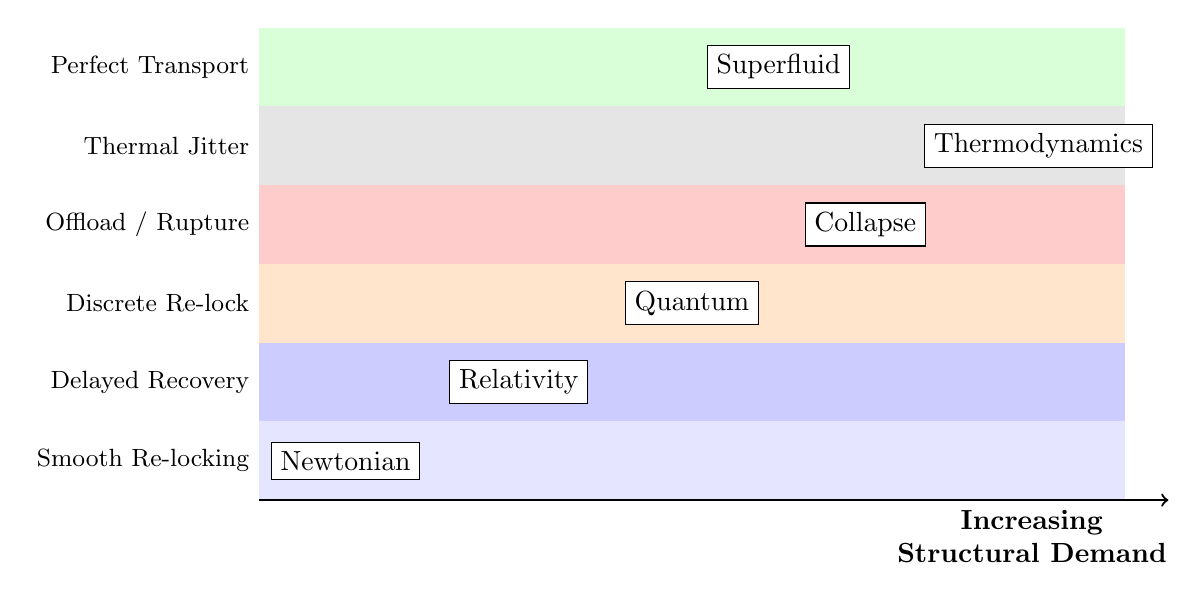
\begin{tikzpicture}[xscale=1.1, yscale=1]

  % Substrate response bands (horizontal)
  \fill[blue!10] (0,0) rectangle (10,1) node[midway,right] {};
  \fill[blue!20] (0,1) rectangle (10,2);
  \fill[orange!20] (0,2) rectangle (10,3);
  \fill[red!20] (0,3) rectangle (10,4);
  \fill[gray!20] (0,4) rectangle (10,5);
  \fill[green!15] (0,5) rectangle (10,6);

  % Y-axis labels (left side)
  \node[anchor=east] at (0,0.5) {\small Smooth Re-locking};
  \node[anchor=east] at (0,1.5) {\small Delayed Recovery};
  \node[anchor=east] at (0,2.5) {\small Discrete Re-lock};
  \node[anchor=east] at (0,3.5) {\small Offload / Rupture};
  \node[anchor=east] at (0,4.5) {\small Thermal Jitter};
  \node[anchor=east] at (0,5.5) {\small Perfect Transport};

  % X-axis line
  \draw[->, thick] (0,0) -- (10.5,0) 
  %node[below right] {\textbf{Increasing Structural Demand}};
  node[pos=0.85, below] {\shortstack{\textbf{Increasing} \\ \textbf{Structural Demand}}};
  
  % Physics regime points (as nodes along ask axis)
  \node[fill=white,draw=black] at (1.0,0.5) {Newtonian};
  \node[fill=white,draw=black] at (3.0,1.5) {Relativity};
  \node[fill=white,draw=black] at (5.0,2.5) {Quantum};
  \node[fill=white,draw=black] at (7.0,3.5) {Collapse};
  \node[fill=white,draw=black] at (9.0,4.5) {Thermodynamics};
  \node[fill=white,draw=black] at (6.0,5.5) {Superfluid};

\end{tikzpicture}
}
\caption{Substrate regime map: each physics domain arises from increasing structural demand on the substrate. Regimes appear at the level of response (vertical) where the substrate begins to express strain.}
\label{fig:substrate_response_corrected}
\end{figure}

\begin{itemize}
    \item \textbf{Left side:} Newtonian zone — wide band, smooth substrate behavior.
    \item \textbf{Middle:} narrowing band through relativistic and quantum regimes.
    \item \textbf{Far right:} collapse threshold and rupture zone.
    \item \textbf{Below band:} thermodynamic offload region (many small asks).
    \item \textbf{Above band:} superfluid transport corridor (fine-tuned match).
\end{itemize}

This figure reinforces the idea that all physics regimes are load zones of a single causal substrate law.

\vspace{1em}

The Regime Map demonstrates that GST does not require separate theoretical foundations for different branches of physics. Each is simply a manifestation of how the substrate balances structural demand against recovery bandwidth under different conditions.
%%%%%%%%%%%%%%%%%%%%%%%%%%%%%%%%%%%%%%%%%%
\section[\appendixname~\thesection]{}
\subsection[\appendixname~\thesubsection]{Ontological Replacements}
\label{app:ontological-replacements}
%%%%%%%%%%%%%%%%%%%%%%%%%%%%%%%%%%%%%%%%%%%%%%%

The General Substrate Theory (GST) does not discard the language of classical or modern physics, but reinterprets its terms through a coherence-based structural ontology. Many concepts that are treated as fundamental entities in existing theories—mass, energy, force, field—are reframed in GST as emergent behaviors of a conserved coherence substrate responding to structural ask.

This appendix provides a reference table of ontological replacements: how key concepts are redefined within the substrate framework.

\renewcommand{\arraystretch}{1.3}
\begin{center}
\begin{tabular}{|p{4cm}|p{7.8cm}|}
\hline
\textbf{Existing Concept} & \textbf{GST Structural Interpretation} \\
\hline
\textbf{Mass} & Persistent coherence deformation held in a phase-locked state; a stored structural demand that resists reconfiguration. \\
\hline
\textbf{Inertia} & Substrate resistance to re-locking a coherent structure across time; scalar pacing drag in response to abrupt structural change. \\
\hline
\textbf{Energy} & Substrate effort required to preserve or change a coherence structure; quantifies tension, phase load, and recovery work. \\
\hline
\textbf{Time} & Scalar tick rhythm—the interval between coherence recovery events; defined by \( t_{\text{tick}} = L_{\text{coh}} / c_s \). \\
\hline
\textbf{Force} & Emergent effect when a system attempts to change structure beyond substrate recovery pacing; re-lock strain expressed over time. \\
\hline
\textbf{Gravity} & Result of equilibrium denial: tension gradient surrounding a phase-saturated region; coherence seeks re-lock in lower tension zones. \\
\hline
\textbf{Spacetime} & Emergent geometry describing relational coherence behavior; not a container, but a projection of pacing and phase continuity. \\
\hline
\textbf{Fields (EM, QFT)} & Stable modal configurations of coherence in transverse or scalar channels; structured behaviors of the substrate under boundary and conservation conditions. \\
\hline
\textbf{Particles} & Quantized outcomes of structural collapse or transport; substrate-localized coherence structures with discrete recovery boundaries. \\
\hline
\textbf{Heat / Entropy} & Accumulated scalar jitter from many unsynchronized asks; substrate offload from coherence saturation. \\
\hline
\textbf{Collapse} & Substrate pacing failure; structure exceeds recovery bandwidth, resulting in rupture, offload, or scalar wave emission. \\
\hline
\textbf{Quantization} & Enforced discreteness due to tick-limited re-locking; not a fundamental ontology, but a constraint on substrate continuity under demand. \\
\hline
\textbf{Vacuum} & Coherence-neutral substrate state; a region of minimal structural commitment, capable of supporting new re-locking or scalar response. \\
\hline
\end{tabular}
\end{center}

\subsubsection*{Interpretive Summary}

GST reinterprets physical entities not as independent primitives, but as the visible expressions of how a conserved substrate balances structural demand with causal capacity. In doing so, it collapses many independent postulates into a single, coherent ontology grounded in:

\begin{itemize}
    \item Pacing constraints (timing and tick)
    \item Structural load and resistance (geometry)
    \item Recovery dynamics (coherence preservation)
    \item Offload and collapse behavior (failure modes)
\end{itemize}

\textit{Where existing physics names effects, GST names causes.}
%%%%%%%%%%%%%%%%%%%%%%%%%%%%%%%%%%%%%%%%%%%
\section[\appendixname~\thesection]{}
\subsection[\appendixname~\thesubsection]{Experimental Discriminants}
\label{app:experimental-discriminants}
%%%%%%%%%%%%%%%%%%%%%%%%%%%%%%%%%%%%%%%%%%%%%%%

A foundational theory must do more than explain — it must predict and risk being wrong. GST makes structural, pacing-based predictions that differ meaningfully from conventional field, particle, or geometric frameworks. This appendix catalogs a set of experimental and observational discriminants that could support or refute key GST claims.

\subsubsection{Rotational Heating as a Proxy for Inertial Drag}

\textbf{Prediction:} Structural inertia arises from scalar re-lock resistance. When a mass-phase object is rotated, the substrate must re-lock the internal coherence structure across time and geometry. If that re-locking is complex, part of the effort will be shed as scalar offload — experienced as measurable rotational heating.

\begin{itemize}
    \item \textbf{Test:} Spin two geometrically distinct but equally massive objects (e.g., one solid sphere and one porous or nanolatticed shell) using identical torque input. Use a calorimetric or IR-based system to measure temperature rise and dissipation rate during and after spin-up.
    \item \textbf{GST Signature:} The more structurally complex object will exhibit greater internal heating due to scalar jitter and offload from inefficient re-locking. This effect is unrelated to surface friction or air resistance and persists in vacuum.
\end{itemize}

\textbf{Interpretive Detail:} In GST, rotational inertia reflects the substrate’s effort to maintain coherent phase alignment across an object undergoing angular acceleration. Structures with greater internal geometric complexity — such as lattice frameworks, porous materials, or composite discontinuities — impose more distributed coherence re-locking demands. As the substrate struggles to re-lock these regions synchronously under rotation, it accumulates pacing strain and sheds excess effort as scalar offload. This offload manifests as internal heating, even in the absence of external friction.

\textit{Rotational heating thus serves as a measurable proxy for inertial drag caused by geometric coherence complexity — a signature predicted by GST but absent in classical mass-only models.}



\subsubsection{Scalar Wave Emission Precursor Events}

\textbf{Prediction:} High-strain collapse events (e.g. supernovae, black hole mergers) should emit scalar coherence waves prior to standard electromagnetic or neutrino signatures.

\begin{itemize}
    \item \textbf{Test:} Analyze multi-detector astrophysical data for pre-event pulses arriving ahead of light and neutrinos — uncorrelated with charged particle behavior.
    \item \textbf{GST Signature:} Early-arriving non-EM signals at or near gravitational-wave frequencies, phase-locked to the collapse geometry.
\end{itemize}

\subsubsection{Quantized Offload Steps in Controlled Collapse}

\textbf{Prediction:} Collapse or emission events involving discrete structural failure (e.g. plasma pinch, fast lattice breakdown) should release energy in quantized bursts, matching envelope-based offload thresholds.

\begin{itemize}
    \item \textbf{Test:} Monitor coherence rupture processes in condensed matter systems (e.g. femtosecond laser disruption, nanostructure failure).
    \item \textbf{GST Signature:} Stepwise energy release at thresholds consistent with \( E = n \cdot \frac{c_t^4}{G} \cdot L_{\text{coh}} \) or multiples of envelope breakdown units.
\end{itemize}

\subsubsection{Coherence Memory Imprint}

\textbf{Prediction:} After a major scalar offload or collapse event, the surrounding substrate should exhibit temporary coherence asymmetries or directional memory.

\begin{itemize}
    \item \textbf{Test:} Interrogate the region around a strong emission source with follow-up pulses; look for angular variation or anisotropic re-lock bias.
    \item \textbf{GST Signature:} Localized directional preference or phase coupling bias that decays over time — not predicted by conventional field relaxation.
\end{itemize}

\subsubsection{Upper Bound on Frequency Emission / Tick Violation Limit}

\textbf{Prediction:} Emissions cannot exceed the substrate's scalar tick rate without collapse or offload; this defines a hard upper bound on frequency.

\begin{itemize}
    \item \textbf{Test:} Attempt to induce ultra-high frequency oscillations beyond \( 1 / t_{\text{tick}} \) in materials or photon sources.
    \item \textbf{GST Signature:} Emission stalls, fragments, or collapses into scalar radiation or chaotic jitter above tick-saturation.
\end{itemize}

\subsubsection*{Interpretive Summary}

\renewcommand{\arraystretch}{1.3}
\begin{center}
\begin{tabular}{|p{4.2cm}|p{7.8cm}|}
\hline
\textbf{Discriminant} & \textbf{GST-Specific Prediction} \\
\hline
Inertial Geometry & Inertia varies with boundary complexity, not just mass. \\
\hline
Scalar Precursor Emission & Coherence rupture precedes photons/neutrinos. \\
\hline
Quantized Collapse Steps & Offload occurs in discrete coherence unit thresholds. \\
\hline
Coherence Memory Effect & Substrate retains directional bias post-rupture. \\
\hline
Frequency Upper Bound & No coherent emission above tick-rate without failure. \\
\hline
\end{tabular}
\end{center}

These discriminants define clear pathways for falsifying GST. Their presence supports the theory’s coherence-pacing framework. Their consistent absence, especially under controlled stress conditions, would challenge its validity.

%%%%%%%%%%%%%%%%%%%%%%%%%%%%%%%%%%%%%%%%%%
%\isPreprints{} % If the paper is ``preprints'', please uncomment this parenthesis.
%\printendnotes[custom] % Un-comment to print a list of endnotes

\reftitle{References}

% Please provide either the correct journal abbreviation (e.g. according to the “List of Title Word Abbreviations” http://www.issn.org/services/online-services/access-to-the-ltwa/) or the full name of the journal.
% Citations and References in Supplementary files are permitted provided that they also appear in the reference list here. 

%=====================================
% References, variant A: external bibliography
%=====================================
% \bibliography{your_external_BibTeX_file}

%=====================================
% References, variant B: internal bibliography
%=====================================

% ACS format
\isAPAandChicago{}{%
\begin{thebibliography}{999}
\bibitem{bush2025}
\textbf{Preprint.} Bush, M. (2025). Quantum Substrate Dynamics (QSD): A Relativistic Field Model of Emergent Mass, Inertia and Gravity. \textit{Preprints}, 2025060988. \url{https://doi.org/10.20944/preprints202506.0988.v1}
% reference
\bibitem{bush-planck-2025}
\textbf{Preprint.} Bush, M. (2025). Planck’s Constant Physically Derived Through Quantum Substrate Dynamics: A Mode-Ratio and Offload-Based Origin for Quantization and Temporal Structure. \textit{Preprints}, 2024010211. \url{https://doi.org/10.20944/preprints202401.0211.v1}
% Reference 
\bibitem{bush-coherence}
Bush, M. The Coherence Envelope: Defining the Minimum Structural Unit of Action in Quantum Substrate Dynamics. {\em Preprints} {\bf 2025}, \url{https://doi.org/10.20944/preprints202506.2353.v1}.
% Reference 
\bibitem{bush-planck-ep}
Bush, M. Planck Energy as Collapse Limit: A Structural Interpretation of $E_P$ in Quantum Substrate Dynamics. {\em Preprints} {\bf 2025}, \url{https://doi.org/10.20944/preprints202507.0080.v1}.
% Reference 
\bibitem{planck1901}
\textbf{Journal article.} Planck, M. (1901). On the Law of Distribution of Energy in the Normal Spectrum. \textit{Annalen der Physik}, 4(553–563). \url{https://doi.org/10.1002/andp.19053221004}
% Reference 
\bibitem{einstein1905} 
\textbf{Journal article.} Einstein, A. (1905). On the electrodynamics of moving bodies. \textit{Annalen der Physik}, 322(10), 891–921. \url{https://doi.org/10.1002/andp.19053221004}
% Reference 
\bibitem{einstein1915} 
\textbf{Journal article.} Einstein, A. (1915). The field equations of gravitation. \textit{Sitzungsberichte der Preussischen Akademie der Wissenschaften}.


\end{thebibliography}
}

% Chicago format (Used for journal: arts, genealogy, histories, humanities, jintelligence, laws, literature, religions, risks, socsci)
\isChicagoStyle{%
\begin{thebibliography}{999}
% Reference 1
%\bibitem[Aranceta-Bartrina(1999a)]{ref-journal}
%Aranceta-Bartrina, Javier. 1999a. Title of the cited article. \textit{Journal Title} %6: 100--10.
% Reference 2

\end{thebibliography}
}{}

% APA format (Used for journal: admsci, behavsci, businesses, econometrics, economies, education, ejihpe, games, humans, ijfs, journalmedia, jrfm, languages, psycholint, publications, tourismhosp, youth)
\isAPAStyle{%
\begin{thebibliography}{999}
% Reference 1
%\bibitem[\protect\citeauthoryear{Azikiwe \BBA\ Bello}{{2020a}}]{ref-journal}
%Azikiwe, H., \& Bello, A. (2020a). Title of the cited article. \textit{Journal Title}, \textit{Volume}(Issue), 
%Firstpage--Lastpage/Article Number.

\end{thebibliography}
}{}

% If authors have biography, please use the format below
%\section*{Short Biography of Authors}
%\bio
%{\raisebox{-0.35cm}{\includegraphics[width=3.5cm,height=5.3cm,clip,keepaspectratio]{Definitions/author1.pdf}}}
%{\textbf{Firstname Lastname} Biography of first author}
%
%\bio
%{\raisebox{-0.35cm}{\includegraphics[width=3.5cm,height=5.3cm,clip,keepaspectratio]{Definitions/author2.jpg}}}
%{\textbf{Firstname Lastname} Biography of second author}

% For the MDPI journals use author-date citation, please follow the formatting guidelines on http://www.mdpi.com/authors/references
% To cite two works by the same author: \citeauthor{ref-journal-1a} (\citeyear{ref-journal-1a}, \citeyear{ref-journal-1b}). This produces: Whittaker (1967, 1975)
% To cite two works by the same author with specific pages: \citeauthor{ref-journal-3a} (\citeyear{ref-journal-3a}, p. 328; \citeyear{ref-journal-3b}, p.475). This produces: Wong (1999, p. 328; 2000, p. 475)

%%%%%%%%%%%%%%%%%%%%%%%%%%%%%%%%%%%%%%%%%%
%% for journal Sci
%\reviewreports{\\
%Reviewer 1 comments and authors’ response\\
%Reviewer 2 comments and authors’ response\\
%Reviewer 3 comments and authors’ response
%}
%%%%%%%%%%%%%%%%%%%%%%%%%%%%%%%%%%%%%%%%%%
\PublishersNote{}
%\isPreprints{} % If the paper is ``preprints'', please uncomment this parenthesis.
\end{document}

